\section{Descripció general de la solució proposada}

A continuació s'exposa l'arquitectura de la plataforma. S'ha tingut en especial consideració l'escalabilitat i l'alta disponibilitat de l'aplicació. És per això que la plataforma consta de diferents nivells desacoblats. Cadascun d'ells ha de funcionar segons els paradigmes de la orientació a serveis en sistemes distribuits, és a dir, cada nivell disposarà de la capacitat d'estar funcionant permanentment i d'escalar de manera independent segons les necessitats. 
També permet minimitzar l'aparició d'elements que puguin esdevenir un "Single Point of Failure". És a dir, elements que en el cas de fallar, tota la plataforma deixaria de donar servei. Finalment, s’aconsegueix detectar i pal·liar colls d'ampolla.

\begin{figure}[H]
    \centering
    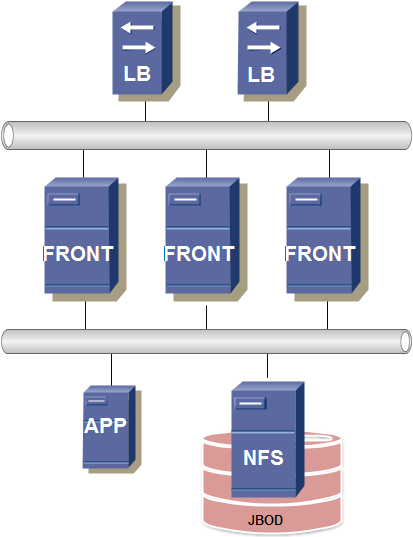
\includegraphics[width=0.7\textwidth]{IM}
    \caption{Arquitectura \label{fig:arquitect}}    
\end{figure}

S'exposaran en primer lloc les capes que es trobin més a prop del client i s'anirà aprofundint.

En primer lloc, hi ha la capa de balanceig de càrrega o "proxy invers". Aquestes màquines rebran peticions web directament dels clients i les enrutaran cap el següent nivell. Tindran la finalitat de prendre la decissió de quina màquina rebrà la petició web. També seran terminadors SSL; actuaran de firewalls, doncs només enrutaran el tràfic per ports (a nivell 4) legítims, i seran la capa visible de l'aplicació a internet.

En segon lloc, hi haurà la capa de "Frontals Web". Aquestes màquines tindran la capacitat de processar la petició web i enrutar aquelles parts que depenguin de codi dinàmic cap a la següent capa. Un cop la següent capa retorni els resultats tindran la capacitat de formatar la presentació de la resposta HTTP. D'altre banda, i com a punt més important, disposaran de gran part del contingut estàtic de l'aplicació. Donat que hi haurà volums molt grans de binaris, s'ha obtat perquè aquesta capa actuï com a cache en disc de les imatges de l'aplicació i del codi estàtic que s'executa al client. Les opciones inicials eren, o bé disposar d'un sistema d'emmagatzematge centralitzat amb totes les imatges o que tots els nodes de la capa disposesin de tots els fitxers estàtics. Donat que es va creure que ambdues eren solucions amb inconvenients insalvables per costos econòmics o per problemes de concurrència, s'ha obtat per la solució de disposar d'alguns fitxers a cada node, maximitzant aquells fitxers que més s'utilitzin.
Amb aquesta decisió s'aconsegueix minimitzar l'espai de disc de les màquines d'aquesta capa, però sense perdre rendiment en quan a latències de xarxa. Val a dir, que permetrà paral·lelitzar l'ample de banda de la xarxa a l'hora d'accedir a les imatges i no saturar la capa d'emmagatzematge. A més a més, permet que l'aplicació escali en capacitat d'usuaris de manera relativament senzilla. Evidentment fins a límits marcats per l'ample de banda de la xarxa de sortida a internet.   

A continuació, hi haurà la capa d'aplicació. Es tracte de nodes que executaran aquelles parts de codi necessaries per desenvolupar la lògica de negoci de l'aplicació. Serà una capa que no tindrà un pes molt important perquè es tracta d'una aplicació amb un ús intensiu en contingut estàtic. No obstant, val a dir que es tractaria d'una capa molt important si l'aplicació web fos d'un altre tipus.
Com a afegit d'aquesta capa hi haurà un servidor d'índexos que permeti cercar imatges eficientment. Es podria contemplar com una altre capa, però s'ha determinat que és una part poc rellevant de la plataforma. És per això que el indexador no disposarà d'alta disponibilitat.

Finalment hi ha la capa d'emmagatzematge. Constarà de dues parts, en primer lloc una solució de cabina de discs SAN que permetrà crear volums a partir dels discs existents així com afegir més discs (JBOD). En segon lloc hi haurà els servidors de storage, els quals seran dos nodes en clúster de nfs per cada cabina de discs provisionada. Les dades en cache dels Frontals seran originalment d'aquests servidors.
